%% ============================================================
%%  IntelliCode Review — Master's Thesis
%%  Safaa Patel, University of Nevada, Reno
%%  Template adapted from UNR Graduate School guidelines
%% ============================================================

\documentclass[12pt, oneside]{report}

%% ---- Packages ----
\usepackage[english]{babel}
\usepackage[margin=1in]{geometry}
\usepackage{setspace}
\usepackage{times}
\usepackage{amsmath, amssymb}
\usepackage{graphicx}
\graphicspath{{figures/}}
\usepackage{xcolor}
\usepackage{listings}
\usepackage{booktabs}
\usepackage{longtable}
\usepackage{array}
\usepackage{multirow}
\usepackage{hyperref}
\usepackage{pdfpages}
\usepackage{acronym}
\usepackage{caption}
\usepackage{subcaption}
\usepackage{float}
\usepackage{enumitem}
\usepackage{fancyhdr}
\usepackage{tocloft}
\usepackage{titlesec}
\usepackage{microtype}
\usepackage{cite}
\usepackage{url}
\usepackage{rotating}
\usepackage{tikz}
\usetikzlibrary{calc, backgrounds}

%% ---- Hyperref Setup — all links BLACK ----
\hypersetup{
    colorlinks=true,
    linkcolor=black,
    citecolor=black,
    urlcolor=black,
    pdftitle={IntelliCode Review: An AI-Powered Platform for Automated Code Quality Analysis with Actionable Feedback},
    pdfauthor={Safaa Patel},
    pdfsubject={Master of Science Thesis, University of Nevada Reno, Computer Science and Engineering},
    pdfkeywords={code quality, static analysis, machine learning, security analysis, defect prediction, software engineering},
    pdflang={en-US},
}

%% ---- Code Listing Style ----
\definecolor{codebg}{rgb}{0.95,0.95,0.95}
\definecolor{codestr}{rgb}{0.63,0.13,0.94}
\definecolor{codecomment}{rgb}{0.25,0.5,0.35}
\definecolor{codekw}{rgb}{0.0,0.0,0.9}

\lstdefinestyle{pythonstyle}{
    language=Python,
    backgroundcolor=\color{codebg},
    basicstyle=\ttfamily\small,
    keywordstyle=\color{codekw}\bfseries,
    stringstyle=\color{codestr},
    commentstyle=\color{codecomment}\itshape,
    numberstyle=\tiny\color{gray},
    numbers=left,
    numbersep=5pt,
    breaklines=true,
    showstringspaces=false,
    frame=single,
    captionpos=b,
}

\lstdefinestyle{jsstyle}{
    language=JavaScript,
    backgroundcolor=\color{codebg},
    basicstyle=\ttfamily\small,
    keywordstyle=\color{codekw}\bfseries,
    stringstyle=\color{codestr},
    commentstyle=\color{codecomment}\itshape,
    numbers=left,
    numbersep=5pt,
    breaklines=true,
    showstringspaces=false,
    frame=single,
    captionpos=b,
}

\lstset{style=pythonstyle}

%% ---- Spacing ----
\doublespacing

%% ---- Header/Footer — UNR requires bottom-center page numbers, no running header ----
\pagestyle{fancy}
\fancyhf{}
\cfoot{\thepage}
\renewcommand{\headrulewidth}{0pt}
\renewcommand{\footrulewidth}{0pt}
%% Redefine plain (used on chapter-opening pages) to match
\fancypagestyle{plain}{%
  \fancyhf{}%
  \cfoot{\thepage}%
  \renewcommand{\headrulewidth}{0pt}%
}

%% ---- Chapter Title Format ----
\titleformat{\chapter}[display]
  {\normalfont\Large\bfseries}{\chaptertitlename\ \thechapter}{20pt}{\Huge}

%% ============================================================
\begin{document}
\begin{titlepage}
\begin{center}

{\Large University of Nevada, Reno}

\vfill

{\LARGE\bfseries IntelliCode Review: An AI-Powered Platform for\\
Automated Code Quality Analysis\\
with Actionable Feedback}

\vfill

{\large A thesis submitted in partial fulfillment of the\\
requirements for the degree of Master of Science\\
in Computer Science and Engineering}

\vfill

{\large by}\\[0.3em]
{\Large Safaa Patel}

\vfill

{\large Dr. Sergiu M. Dascalu, Advisor}

\vfill

{\large May, 2026}

\end{center}
\end{titlepage}

%% ---- Copyright Page ----
\clearpage
\thispagestyle{empty}
\vspace*{\fill}
\begin{center}
\textcopyright\ by Safaa Patel\\
All Rights Reserved
\end{center}
\vspace*{\fill}

%% ---- Approval Page (inserted from PDF) ----
\clearpage
\includepdf[
    pages=1,
    fitpaper=true,
    pagecommand={\thispagestyle{empty}}
]{approv.pdf}

%% ---- Front Matter Numbering ----
\pagenumbering{roman}
\setcounter{page}{1}

%% ============================================================
%%  ABSTRACT
%% ============================================================
\clearpage
\chapter*{Abstract}
\addcontentsline{toc}{chapter}{Abstract}

Most developers know, at some level, that code quality deteriorates if it is not actively
managed. The tools available to help are fragmented: a security scanner here, a complexity
metric there, a style checker whose warnings most teams quietly learn to ignore. Assembling
a complete picture of a codebase's health from these disconnected sources is tedious, and
the results rarely guide concrete action. Manual code review, the traditional fallback,
is slow, inconsistent, and limited by the expertise and attention of whoever happens
to be reviewing on a given day.

This thesis describes the design, implementation, and evaluation of \textit{IntelliCode
Review}, a web-based platform that consolidates twelve code quality analysis dimensions
into a single, interactive application. The system accepts Python, JavaScript, TypeScript,
and Java source code and returns a quality report covering security vulnerabilities,
cyclomatic and cognitive complexity, bug probability, code clones, refactoring
opportunities, dead code, technical debt, documentation coverage, performance hotspots,
dependency coupling, and readability, all in under two seconds. Four of the twelve
dimensions are driven by trained machine learning models; the remaining eight are
deterministic AST-based analysers that produce reproducible results without probabilistic
uncertainty. The deterministic modules are validated for pipeline correctness but not
for detection accuracy; precision and recall evaluations for those components remain
future work.

The machine learning results are uneven, and the failures are as informative as the
successes. A peer-review audit caught a label-leakage defect in the original complexity
model, which had produced a spurious $R^2 = 1.000$ by using a target analytically
derivable from the input features. The corrected XGBoost complexity predictor reaches
$R^2 = 0.676 \pm 0.063$ and Pearson $r = 0.980$ against SonarQube. Complexity ranking
holds in cross-project evaluation, transferring to nine of ten held-out repositories (mean
Spearman $\rho = 0.795 \pm 0.186$). The one failure is \texttt{tiangolo/fastapi}, a
decorator-heavy, Pydantic-style codebase outside the training distribution.

The security ensemble (Random Forest + 1D CNN) reaches in-distribution AUC
$= 0.963 \pm 0.012$ on 4,286 labelled samples. Cross-project evaluation collapses to
AUC $= 0.494 \pm 0.189$, essentially at chance. The training data over-represents CVE patterns from
a narrow set of vulnerability categories; repositories with different exposure profiles
produce feature distributions outside that training envelope. High in-distribution AUC
is not evidence of transferability, and this result is the clearest demonstration of that.

The bug predictor reaches AUC $= 0.676 \pm 0.038$ on a standard random split, consistent with the JIT defect prediction literature. A strict temporal split (train
on the earliest 80\% of commits, test on the most recent 20\%) gives AUC $= 0.460$,
below chance. Static file-level metrics do not capture how a codebase evolves; training
on commits that post-date a bug fix produces temporal leakage that inflates the random-split
figure. Under a forward-looking evaluation, the module provides no reliable bug forecast.

The pattern classifier, after removing 14 leaky features that directly encoded the label
assignment rules, was retrained on 22 non-leaky structural AST features using XGBoost,
achieving a debiased CV F1 of $0.653 \pm 0.017$ (test F1 $= 0.688$, AUC $= 0.848$, accuracy $= 67.1\%$). The original 26-feature
model's F1 of 0.804 included $+0.082$ of circular label supervision (Wilcoxon $p=0.031$);
that gap is now documented and the debiased model is the production checkpoint.

The evaluation protocol may be the most potentially transferable contribution. Multi-seed variance,
LOPO benchmarks, temporal splits, residual conformal intervals, and a SonarQube
calibration together expose generalisation limits that a single held-out test split would
not catch. A lightweight peer-based evaluation with four graduate students provided
preliminary usability feedback; a controlled study with professional developers remains
future work. The prototype needs no infrastructure beyond a local Python environment and
a browser.

%% ============================================================
%%  DEDICATION
%% ============================================================
\clearpage
\chapter*{Dedication}
\addcontentsline{toc}{chapter}{Dedication}

I dedicate this thesis to my family, who made graduate school possible by believing in me
when I did not always believe in myself.

%% ============================================================
%%  ACKNOWLEDGMENTS
%% ============================================================
\clearpage
\chapter*{Acknowledgments}
\addcontentsline{toc}{chapter}{Acknowledgments}

My advisor, Dr Sergiu Dascalu, improved this work in ways large and small. His feedback
pushed the evaluation from a single train-test split to the multi-methodology protocol
described in Chapter~\ref{ch:eval}, and his patience with the iterations in between was
genuinely appreciated.

The UNR Department of Computer Science and Engineering provided the computing resources
and coursework that gave this project its foundations.

The open-source maintainers behind Python, FastAPI, React, XGBoost, scikit-learn, and
PyTorch did most of the hard work this thesis builds on. The maintainers of Django, Flask,
requests, and pip gave me real training data simply by keeping their commit histories
public.

My family kept me sane. That is not a small thing.

%% ============================================================
%%  TABLE OF CONTENTS / FIGURES / TABLES
%% ============================================================
\clearpage
\tableofcontents
\clearpage
\listoftables
\clearpage
\listoffigures


%% ============================================================
%%  MAIN CONTENT
%% ============================================================
\clearpage
\pagenumbering{arabic}
\setcounter{page}{1}
%% ============================================================
\chapter{Introduction}
\label{ch:intro}
%% ============================================================

\section{Problem Statement}
\label{sec:problem}

Software development teams have always understood that code quality matters: defects caught in review are cheaper than defects caught in production. The National Institute of Standards and Technology estimated software defect costs at \$60 billion per year in the US economy alone~\cite{nist2002}, and subsequent studies confirm that defect density correlates with code complexity~\cite{mccabe1976}. The knowledge exists; the difficulty lies in applying it at the pace modern development demands.

Manual code review, where a human peer reads changes and comments before they merge,
remains the industry-standard quality gate. It is valuable, but it has
well-documented structural weaknesses. Review quality is inconsistent: the same patch
may receive a thorough critique one day and a perfunctory approval the next, depending
on reviewer load, expertise, and attention~\cite{bacchelli2013, mcintosh2016}.
Reviewers tend to be better at catching style violations than at detecting logical bugs
or security vulnerabilities, particularly in unfamiliar parts of the codebase~\cite{fagan1976}.
As teams grow and deployment cadences accelerate, the reviewer-to-change-set ratio
worsens, and the review process becomes a bottleneck rather than a safety net.

Automated static analysis tools (Pylint, Flake8, Bandit, and their counterparts in other language ecosystems) address some of this gap by running fast, deterministic
checks that do not depend on human attention. They catch obvious issues: undeclared
variables, imports that shadow builtins, string-formatted SQL queries. But they are
fundamentally limited by their architecture. They match code against a fixed rule set;
they do not adapt to the patterns that have historically caused bugs in a particular
project, cannot estimate the probability that a given commit will introduce a regression,
and do not produce a single integrated quality score that a developer can act on
immediately. The output of running three different static analysis tools is three
separate lists of warnings in three different formats, with no guidance on which to
prioritise.

Machine learning offers a path beyond this limitation: models trained on commit histories can learn which code patterns precede bugs; models trained on CVE-annotated code generalise vulnerability patterns beyond fixed rules; regression models predict cognitive complexity from structural metrics. The challenge is assembling these capabilities into a tool a solo developer can run without infrastructure or specialist expertise.

\section{Proposed Solution}
\label{sec:solution}

IntelliCode Review is the response to the challenge stated above: a web-based platform
that consolidates twelve code quality analysis dimensions into a single interactive
application, trained on real open-source code and evaluated against the same cross-project
and temporal standards applied to published defect predictors.

The primary contribution of this thesis is an evaluation protocol for ML-based code
analysis that takes generalisation seriously: multi-seed variance, leave-one-project-out
benchmarks, temporal splits, residual conformal intervals, and a SonarQube calibration
designed to catch leakage rather than confirm it. That protocol is the transferable
result. IntelliCode Review, a twelve-dimension analysis platform backed by those same models, is what makes the evaluation concrete. Without a working system, the
protocol has nothing to evaluate; without the protocol, the system's claims are no
more credible than the optimistic benchmarks in the papers it cites.

The secondary contribution is the system itself: broader dimension coverage in a
self-contained tool than any existing open-source alternative, with an interface
designed around the constraint that findings ignored are findings wasted.

The models are not individually state-of-the-art. The evaluation is the point.

This thesis argues that rigorous evaluation, not model sophistication, is the unsolved problem in applied ML for software engineering. Building the system is the tractable part; knowing what it actually does in conditions that approximate deployment is harder and, for a practitioner deciding whether to trust a tool, more useful. Coverage and speed only matter if developers actually consult the results: a finding that takes thirty seconds arrives too late, and a security alert that requires switching tools gets dismissed. The system was built around that constraint.

\section{Research Questions}
\label{sec:rq}

Three questions guide the work:

\begin{description}
  \item[RQ1] Does a unified ML-augmented platform cover a broader set of code
    quality analysis dimensions than traditional single-purpose static analysis
    tools, and do the individual modules produce technically correct outputs on
    verified test cases? The empirical motivation is that developers using fragmented
    tooling systematically under-examine dimensions not covered by their default
    linter~\cite{johnson2013}: a security-only tool produces no complexity signal;
    a complexity-only tool produces no dead-code or clone signal. A unified platform
    removes the decision of which tool to run, which changes what gets examined.
    Coverage is measured by dimension count relative to tools operating under comparable infrastructure constraints (no dedicated server, no external service account); correctness is measured by end-to-end functional testing against hand-labelled inputs.
    Whether broader coverage translates to better developer outcomes is not
    investigated here and remains an open empirical question.
  \item[RQ2] How do the chosen machine learning architectures (XGBoost, RF+CNN
    ensemble, LR+XGBoost ensemble, calibrated Random Forest) perform on each of the
    four trained quality tasks (security, complexity, bug prediction, pattern
    recognition) when trained on real open-source data and evaluated under
    cross-project and temporal protocols?
  \item[RQ3] Can the system be implemented as a practical, self-contained web
    application with response times fast enough for interactive developer workflows,
    without requiring server infrastructure or external service accounts?
\end{description}

\section{Scope and Limitations}
\label{sec:scope}

IntelliCode Review accepts Python, JavaScript, TypeScript, and Java for direct analysis.
Python receives the full twelve-model treatment including ML-based security, complexity,
bug prediction, and pattern recognition. JavaScript, TypeScript, and Java receive
deterministic security scanning (eight vulnerability categories via language-specific
regex rules) and cyclomatic complexity via tree-sitter AST parsers; the trained ML
models do not run for these languages. The repository scanner additionally recognises
twelve further languages (C, C++, Go, Rust, Ruby, PHP, Swift, Kotlin, Scala, R, Dart,
and Shell) for file-level metrics only. The platform integrates with GitHub for repository
scanning: users can connect a personal access token to trigger batch scans of entire
repositories from the Repositories page. The API also accepts optional git metadata
(code churn, author count, file age, past bug count, commit frequency) to augment bug
prediction for Python files.

All four ML models are trained on real open-source code drawn from 33 repositories
across five domains: 4,286 security samples from CVE-annotated commits, 3,015
complexity samples, 8,668 bug-labelled commits, and 6,200+ pattern examples covering
web frameworks, data science libraries, CLI tools, testing infrastructure, and
async networking libraries. Generalisation to unseen production codebases is limited by
that training distribution; model probabilities are risk indicators, not verdicts.

Readers primarily interested in the engineering details will find them in Chapters~\ref{ch:design} and~\ref{ch:demo}; readers primarily interested in the evaluation methodology will find the core argument in Chapter~\ref{ch:eval}.

\section{Thesis organization}
\label{sec:organization}

Chapter~\ref{ch:background} covers the technical background: code review, static
analysis, complexity metrics, and the machine learning methods the platform uses.
Chapter~\ref{ch:related} positions IntelliCode Review relative to existing tools and
research, from traditional linters to deep learning vulnerability detectors.
Chapter~\ref{ch:motivation} argues the case for the design and states the five concrete
goals. Chapter~\ref{ch:design} describes the architecture and implementation in detail.
Chapter~\ref{ch:demo} walks through the interface with three worked demonstration
scenarios. Chapter~\ref{ch:eval} presents the evaluation methodology and results,
including the audit correction, LOPO benchmarks, feature ablation study, and adversarial robustness analysis. Chapter~\ref{ch:conclusion}
summarises the contributions, answers the research questions, and discusses future work.

%% ============================================================
\chapter{Background}
\label{ch:background}
%% ============================================================

\section{Code Review in Software Engineering}
\label{sec:bg-codereview}

Code review is the examination of source code by someone other than the original author,
with the goal of finding defects, improving quality, and spreading knowledge within a
team~\cite{fagan1976}. Fagan's formal inspection process at IBM in the 1970s was the
precursor to modern lightweight peer review. The current dominant form is asynchronous
pull-request review on platforms such as GitHub, GitLab, and Gerrit~\cite{bacchelli2013}.

Empirical studies of review in practice find that reviewers focus on understandability,
coding conventions, and functional correctness~\cite{bacchelli2013}. Security defects
and performance issues get caught far less often~\cite{mcintosh2016}, partly because they demand domain expertise that not every reviewer has and partly because they are harder to spot by reading code than by running it. This is the structural weakness.
That gap, between what manual review
reliably catches and what actually matters for code health, is the problem automated
analysis is meant to close.

\subsection{Pull-request-based review}

Modern teams submit code changes as pull requests, reviewed by peers before merging.
This creates a natural insertion point for automated tooling: the analysis can run on
the PR before any human reviewer opens the diff, filtering out mechanical issues so
that reviewer attention is spent on logic, design, and correctness. IntelliCode Review
is intended for this workflow: a developer submits a file, receives an automated quality report, addresses the findings, and only then asks a peer to review.

\subsection{Cost of Poor Code Quality}

Technical debt, the implied cost of choosing a quick solution over a better one, accumulates with poor code quality. The SQALE (Software Quality
Assessment based on Lifecycle Expectations) methodology~\cite{letouzey2012} quantifies
technical debt in person-hours required to fix each quality issue category. IntelliCode
Review implements a SQALE-inspired debt estimator that aggregates findings from security,
complexity, clone detection, dead code, and refactoring models into a single debt report.

\section{Static Analysis}
\label{sec:bg-static}

Static analysis examines source code without executing it. It encompasses a broad range
of techniques from simple lexical pattern matching to full dataflow and taint analysis.

\subsection{Lexical and Syntactic Analysis}

The simplest form of static analysis scans source code as text, searching for known
dangerous patterns using regular expressions. Tools such as Bandit for Python use this
approach to flag uses of \texttt{eval()}, hardcoded passwords, and insecure deserialization.
IntelliCode Review's security pattern scanner (\texttt{security\_patterns.py}) implements
a curated set of regular expressions covering SQL injection, command injection, path
traversal, hardcoded secrets, weak cryptography, insecure deserialization, code injection,
and XXE vulnerabilities.

\subsection{Abstract Syntax Tree Analysis}

An abstract syntax tree (AST) captures grammatical structure without syntactic noise.
Python's standard library provides the
\texttt{ast} module, which parses source code into an AST and enables tree-walking
visitors. The system leans heavily on AST analysis: the \texttt{ASTExtractor}
class extracts features including function definitions, call sites, import statements,
string literals, class hierarchies, and control flow constructs. Seven of the twelve
models (clone detection, refactoring, dead code, documentation quality, performance,
dependency, and readability) are implemented as AST visitors or pattern matchers.

\subsection{Complexity Metrics}

The field has settled on four main metrics for measuring complexity:

\begin{description}
  \item[Cyclomatic Complexity (McCabe)~\cite{mccabe1976}] Counts the number of linearly
    independent paths through a program's control flow graph. Formally, $V(G) = E - N + 2P$
    where $E$ is edges, $N$ is nodes, and $P$ is connected components.
  \item[Cognitive Complexity~\cite{campbell2018}] A successor metric that penalizes
    nested control structures more heavily, arguing that nesting is a stronger predictor
    of comprehension difficulty than raw path count.
  \item[Halstead Metrics~\cite{halstead1977}] Derive a family of metrics (volume, difficulty,
    effort, predicted bugs) from counts of operators and operands in the source code.
  \item[Maintainability Index~\cite{oman1992}] A composite metric (0--100 scale) combining
    Halstead volume, cyclomatic complexity, and source lines of code, widely used by
    tools such as Visual Studio.
\end{description}

IntelliCode Review computes all four families of metrics in \texttt{code\_metrics.py}.
After correcting a label-leakage defect in the original implementation (see
Section~\ref{sec:eval-methodology}), the XGBoost complexity model uses a 15-dimensional
feature vector with cognitive complexity as the prediction target rather than as a feature.

\section{Machine Learning for Code Analysis}
\label{sec:bg-ml}

\subsection{Defect Prediction}

Defect prediction work has been running since roughly 2000~\cite{nagappan2005, zimmermann2007}.
Early models used product metrics (lines of code, complexity) and process metrics like code churn and developer experience as features for logistic regression or na\"ive Bayes.
Later work showed that random forests~\cite{lessmann2008}, support vector machines, and
neural networks could push accuracy further, though the gains varied widely by dataset.

IntelliCode Review's bug predictor follows this tradition, combining static code metrics
with optional git metadata (code churn, author count, file age, past bug count, commit
frequency) in a Logistic Regression + XGBoost ensemble, where the gradient-boosted tree
component benefits from early stopping regularisation (best iteration at epoch 97).

\subsection{Vulnerability Detection}

ML-based vulnerability detection accelerated after the release of labelled datasets:
Devign~\cite{zhou2019}, D2A, and CodeXGLUE. Approaches range from simple TF-IDF
bag-of-tokens classifiers to graph neural networks over code property
graphs~\cite{yamaguchi2014}, with graph-based methods generally performing better on
tasks that require interprocedural reasoning.

The security component uses a practical two-component ensemble: (1) a Random Forest classifier
operating on a 25-dimensional feature vector (17 code metrics plus 8 security-specific counters
covering dangerous imports, dangerous calls, long string literals, scanner findings at each
severity level, try-block count, string literal count, and call site count), and (2) a 1D
Convolutional Neural Network operating on token ID sequences of length 512.
The ensemble combines both predictions via a weighted average ($w_{RF}=0.55$, $w_{CNN}=0.45$);
these weights were fixed a priori based on validation-set precision-recall balance rather than
optimised by grid search, so they do not introduce an additional tuning degree of freedom.

\subsection{Code Embeddings and Pre-Trained Models}

Pre-trained transformer models for code --- CodeBERT~\cite{feng2020}, GraphCodeBERT~\cite{guo2021}, and CodeT5~\cite{wang2021} --- established strong baselines across vulnerability detection, clone detection, code summarization, and defect prediction.

A CodeBERT-based approach was evaluated for pattern recognition and rejected in favour of a calibrated XGBoost classifier on a 22-dimensional debiased AST feature vector, primarily to avoid the $\sim$500\,MB model download and GPU requirement. After removing 14 leaky features that encoded the label rules directly, the debiased CV F1 is $0.653 \pm 0.017$ (test F1 $= 0.688$, AUC $= 0.848$). Section~\ref{ssec:pattern} details this design.

\subsection{Ensemble Methods}

Ensemble methods combine multiple base learners to reduce variance and improve
generalization. Random forests are a bagging ensemble of decision trees; gradient
boosted trees (XGBoost~\cite{chen2016}) train trees sequentially, each correcting
the errors of the previous. XGBoost handles complexity prediction here, chosen for its strong performance on tabular regression and resistance to
overfitting. The security and bug prediction models both use two-component ensembles
(RF/CNN and LR/XGBoost respectively) to combine complementary representations.

%% ============================================================
\chapter{Related Work}
\label{ch:related}
%% ============================================================

\section{Automated Code Review Systems}
\label{sec:rel-review}

Automated code review is not a single thing. It covers rule-based linters, statistical
defect predictors, graph neural networks over code property graphs, and commercial
platforms that mix several of these. This chapter covers the work most directly relevant
to IntelliCode Review and explains where this thesis sits relative to each tradition.

\subsection{Traditional Static Analysis Tools}

Pylint~\cite{pylint}, Flake8, and mypy represent the mainstream of Python static analysis.
Pylint checks for coding conventions, error detection, and refactoring suggestions through
a rule-based system. Flake8 wraps pycodestyle, pyflakes, and McCabe complexity into a
lightweight linter. Bandit~\cite{bandit} focuses exclusively on security, scanning for
dangerous function calls, insecure defaults, and known vulnerability patterns using
a plugin architecture.

The limitation is the rule set itself: these tools can only detect what their authors
anticipated. They do not learn from the codebase being analysed, do not predict future
bugs, and produce no integrated score across multiple dimensions. IntelliCode Review
augments rule-based analysis with ML models that capture patterns too context-dependent
to express as fixed rules.

SonarQube~\cite{sonarqube} is a commercial platform offering multi-language static analysis
with quality gates, technical debt tracking, and CI/CD integration. It is the closest
commercial analogue to IntelliCode Review. However, SonarQube uses rule-based analysis
rather than trained ML models for most of its checks, requires significant infrastructure
(a Java server, database), and is primarily oriented toward team-level dashboards rather
than individual developer feedback.

\subsection{CodeClimate and Similar Platforms}

CodeClimate provides automated code review for GitHub repositories, computing a
maintainability score based on duplication, complexity, and code smells. Like SonarQube,
it is rule-based and lacks ML-based defect prediction. IntelliCode Review differs by
incorporating trained models for security, bugs, and complexity, and by running as a
self-contained prototype that requires no external service account or API key.

Amazon CodeGuru Reviewer~\cite{codeguru} uses ML to detect resource leaks, concurrency issues, and security vulnerabilities in Java and Python code through pull request integration. GitHub Advanced Security~\cite{ghadvancedsecurity} (formerly LGTM) applies CodeQL dataflow analysis across multiple languages. DeepScan and Codacy offer ML-assisted analysis as cloud services. All three have access to proprietary training data and production-scale infrastructure that a research prototype cannot match.

IntelliCode Review sits in a different position. It is self-contained, runs without cloud dependencies, and reports cross-project evaluation results — including the failures — rather than presenting only in-distribution benchmarks. The dimension-coverage comparison in Table~\ref{tab:coverage} is most meaningful when read against the open-source tools Bandit, Pylint, Radon, and SonarQube Community Edition, all of which run under comparable infrastructure constraints.

\section{Defect Prediction}
\label{sec:rel-defect}

\subsection{Metric-Based Approaches}

Nagappan and Ball~\cite{nagappan2005} demonstrated that relative code churn metrics predict
defect density with high accuracy across Windows Server 2003 components. Their work
established code churn (lines added, deleted, and changed between revisions) as a key
predictor, which IntelliCode Review incorporates as an optional feature in its bug
predictor. Zimmermann et al.~\cite{zimmermann2007} extended defect prediction to use
network analysis of code dependencies, finding that highly connected components tend to
have more defects.

\subsection{Machine Learning Approaches}

Lessmann et al.~\cite{lessmann2008} compared 22 classifiers for defect prediction and found no single classifier consistently dominates, motivating ensemble approaches. IntelliCode Review's LR + XGBoost ensembling pairs calibrated probability estimates with XGBoost's nonlinear interactions. Kamei et al.~\cite{kamei2013} introduced just-in-time defect prediction operating on individual commits; the IntelliCode Review bug predictor borrows git-level metadata (churn, author count, commit frequency) from this tradition, though a strict temporal split reveals that git metadata does not overcome distribution shift.

\subsection{Deep Learning for Defect Prediction}

Li et al.~\cite{li2017} showed that CNN models over source token sequences capture structural information without manual feature engineering — the motivation for IntelliCode Review's 1D CNN security component. Zhou et al.~\cite{zhou2019} introduced Devign, a GNN approach over joint code property graphs for C/C++ vulnerability detection; the principle of combining structural and lexical views is reflected in the RF+CNN ensemble.

\section{Code Clone Detection}
\label{sec:rel-clone}

Roy and Cordy~\cite{roy2007} defined four clone types; the IntelliCode Review clone detector covers Types 1--3 using normalised AST representation and TF-IDF cosine similarity. SourcererCC~\cite{sajnani2016} scaled TF-IDF bag-of-tokens to billion-line codebases; IntelliCode Review uses a lighter in-memory version appropriate for single-file snippet analysis.

\section{Code Readability and Maintainability}
\label{sec:rel-readability}

Buse and Weimer~\cite{buse2010} developed a machine learning model for predicting code
readability based on local features (identifier length, keyword density, line length,
indentation consistency). Their model achieved strong correlation with human readability
judgments. IntelliCode Review's readability scorer implements a multi-dimensional scoring
approach inspired by this work, evaluating naming conventions, comment density, structural
consistency, and cognitive load.

\section{Pre-Trained Models for Code}
\label{sec:rel-pretrained}

Feng et al.~\cite{feng2020} introduced CodeBERT, achieving strong results on code search, documentation generation, and clone detection. Its infrastructure requirements (~500\,MB weights, GPU inference) are impractical for a locally-deployed tool targeting solo developers. A calibrated XGBoost classifier on 22 debiased structural AST features satisfies the latency budget ($<$200\,ms on CPU); the debiased model achieves AUC $= 0.848$ and CV F1 $= 0.653$. The original 26-feature numbers (AUC $= 0.969$, F1 $= 0.804$) were inflated by label leakage and are not reported as primary results.

\section{Developer tool adoption and alert fatigue}
\label{sec:rel-adoption}

The developer tool adoption literature provides empirical grounding for several design
decisions in IntelliCode Review. Johnson et al.~\cite{johnson2013} surveyed professional
developers about their reasons for not using static analysis tools and found three
dominant barriers: too many false positive warnings, difficulty customising the tool to
their workflow, and a perceived mismatch between warning categories and actual bugs they
cared about.

Christakis and Bird~\cite{christakis2016} found that 91\% of developers who stopped using a static analysis tool cited false positives as the primary reason; even a 1-in-5 false positive rate led most to dismiss all output. This \textit{alert fatigue} effect directly informed IntelliCode Review's design: the security model uses an operating threshold of 0.050 to favour precision over recall, findings are grouped by root cause rather than line number, and the bug predictor surfaces its three evaluation-protocol AUC values to discourage over-reliance on the raw probability. Kononenko et al.~\cite{kononenko2016} found that unclear or unprioritised findings are the primary cause of review feedback being ignored, motivating the Fix Guide's before/after format and effort estimates.

\section{Integrated developer productivity tools}
\label{sec:rel-idt}

GitHub Copilot and Amazon CodeWhisperer address code \textit{generation}: suggesting
completions, functions, and boilerplate. They do not analyse existing code for defects.
IntelliCode Review is in a different position: it does not write code, but scrutinises what is already there.

DeepCode (now Snyk Code) uses an ML pipeline similar in spirit to IntelliCode Review's RF+CNN ensemble but is almost entirely security-focused and publishes no cross-project or temporal evaluation results in peer-reviewed venues. IntelliCode Review distributes attention across twelve dimensions and reports LOPO AUC = 0.494 — transparency that commercial tools do not provide even when their proprietary in-distribution benchmarks show higher absolute performance.

\subsection*{Evaluation practice and the field consensus}

The majority of defect prediction and vulnerability detection papers report AUC or F1 on a single random split. Shepperd et al.~\cite{shepperd2014} and Tantithamthavorn et al.~\cite{tantithamthavorn2016} showed that random splits inflate performance by allowing training on future commits; Menzies et al.~\cite{menzies2011} documented severe cross-project degradation. Cross-project defect prediction reliably falls below random-split performance --- Zimmermann et al.~\cite{zimmermann2007} found 0\% accuracy on cross-project transfer for some tasks --- and random splits overestimate temporal AUC by 10--30\% for static-metric JIT models~\cite{kamei2013}. Label quality, not model capacity, is typically the binding constraint.

This thesis treats temporal leakage and distribution shift as primary results, not footnotes. IntelliCode Review's LOPO results (security AUC $= 0.494$, bug predictor temporal AUC $= 0.460$) are the expected consequence of applying ML to code quality under realistic constraints. PIFF, SAEF, LAMV, and TDCP address distinct categories of this reporting gap; no prior work in this survey applies all four.

%% ============================================================
\chapter{Motivation and Proposed Solution}
\label{ch:motivation}
%% ============================================================

\section{Motivation}
\label{sec:motivation}

Three problems in current code quality tooling shaped the design of IntelliCode Review.
Each one is a real friction point, not an abstract concern.

\textbf{Fragmentation.} Getting comprehensive Python feedback today means running Pylint
for style, Bandit for security, radon for complexity, vulture for dead code, and possibly
a paid service for technical debt. Each tool has a different configuration format, a
different severity scale, and a different output schema. Putting those results together
takes work that most developers skip, so parts of the picture go unexamined by default.

\textbf{The ceiling on rule-based detection.} Rules catch what their authors anticipated.
Code quality issues are often context-dependent: combinations of features that are
individually harmless can together indicate elevated risk in ways that are hard to
express as fixed patterns. ML models trained on labelled examples of vulnerable or
complex code can capture those distributional patterns, at the cost of requiring
training data and accepting probabilistic outputs.

\textbf{Adoption.} As established in Section~\ref{sec:rel-adoption}, developers abandon tools that produce excessive false positives or demand non-trivial configuration~\cite{johnson2013, christakis2016}. Speed and low friction are not polish; they determine whether analysis results are ever seen.

\section{Design Goals}
\label{sec:goals}

Those three problems translate into five concrete goals.
\textbf{Comprehensiveness:} cover twelve quality dimensions in one request — no tool-switching, no reconciliation.
\textbf{ML augmentation:} at least three components use trained models to capture distributional patterns that fixed rules cannot anticipate.
\textbf{Speed:} full 1000-line analysis within two seconds; a fast path below 500\,ms for CI pre-commit hooks.
\textbf{Persistence:} analysis history, custom rules, and repository configurations survive browser sessions without a backend database.
\textbf{Actionability:} every finding carries a severity classification, a CWE identifier, and a before/after remediation snippet; a finding without a concrete fix is only marginally better than no finding at all.

\section{System Overview}
\label{sec:overview}

Figure~\ref{fig:architecture} shows the high-level architecture of IntelliCode Review,
which is structured across three tiers. The browser-based frontend is a React 18 SPA
where developers submit code, browse results across fourteen analysis tabs, track quality
trends on the Analytics page, and compare two snippets side by side. The browser stores all analysis history in \texttt{localStorage}, with no backend database required.

The Python FastAPI backend receives requests and dispatches them to the appropriate
model classes in parallel. It exposes over twenty endpoints: the full combined analysis
at \texttt{/analyze}, twelve specialised model endpoints, a Server-Sent Events streaming
endpoint at \texttt{/analyze/stream} for progressive results, a fast sub-500\,ms path
at \texttt{/analyze/quick}, and utility endpoints for statistics, feedback collection,
and cache management.

The ML layer consists of twelve model classes. Four of them (security, complexity, bug prediction, and pattern recognition) use trained checkpoints loaded from disk at startup. The remaining eight are deterministic AST-based analysers that produce
reproducible results without probabilistic uncertainty.

\begin{figure}[H]
\centering
\resizebox{\linewidth}{!}{%
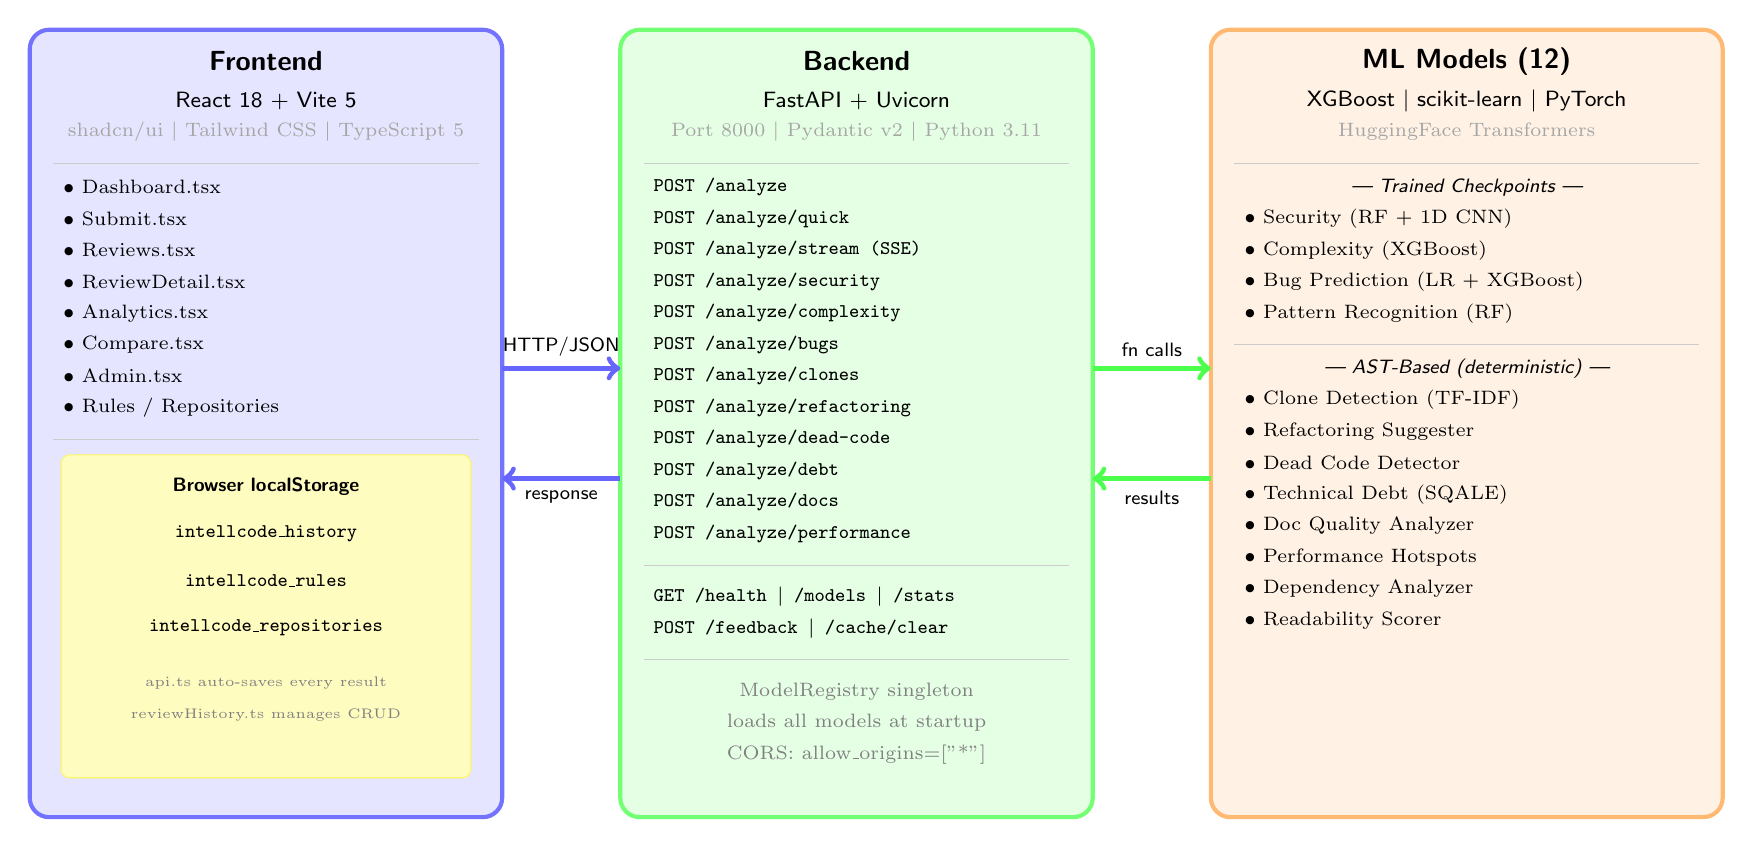
\begin{tikzpicture}[font=\sffamily\footnotesize]

%% --- Frontend box -------------------------------------------
\filldraw[fill=blue!10, draw=blue!55, line width=1.5pt, rounded corners=7pt]
  (-3.0,-5.0) rectangle (3.0,5.0);
\node[font=\sffamily\bfseries\normalsize] at (0,4.6) {Frontend};
\node at (0,4.1) {React 18 + Vite 5};
\node[font=\scriptsize, text=gray!70] at (0,3.7) {shadcn/ui \textbar\ Tailwind CSS \textbar\ TypeScript 5};
\draw[gray!40, thin] (-2.7,3.3) -- (2.7,3.3);
\node[font=\scriptsize, anchor=west] at (-2.7, 3.0) {$\bullet$~Dashboard.tsx};
\node[font=\scriptsize, anchor=west] at (-2.7, 2.6) {$\bullet$~Submit.tsx};
\node[font=\scriptsize, anchor=west] at (-2.7, 2.2) {$\bullet$~Reviews.tsx};
\node[font=\scriptsize, anchor=west] at (-2.7, 1.8) {$\bullet$~ReviewDetail.tsx};
\node[font=\scriptsize, anchor=west] at (-2.7, 1.4) {$\bullet$~Analytics.tsx};
\node[font=\scriptsize, anchor=west] at (-2.7, 1.0) {$\bullet$~Compare.tsx};
\node[font=\scriptsize, anchor=west] at (-2.7, 0.6) {$\bullet$~Admin.tsx};
\node[font=\scriptsize, anchor=west] at (-2.7, 0.2) {$\bullet$~Rules / Repositories};
\draw[gray!40, thin] (-2.7,-0.2) -- (2.7,-0.2);
\filldraw[fill=yellow!25, draw=yellow!60, rounded corners=3pt]
  (-2.6,-0.4) rectangle (2.6,-4.5);
\node[font=\sffamily\bfseries\scriptsize] at (0,-0.8) {Browser localStorage};
\node[font=\scriptsize\ttfamily] at (0,-1.4) {intellcode\_history};
\node[font=\scriptsize\ttfamily] at (0,-2.0) {intellcode\_rules};
\node[font=\scriptsize\ttfamily] at (0,-2.6) {intellcode\_repositories};
\node[font=\tiny, text=gray] at (0,-3.3) {api.ts auto-saves every result};
\node[font=\tiny, text=gray] at (0,-3.7) {reviewHistory.ts manages CRUD};

%% --- Backend box --------------------------------------------
\filldraw[fill=green!10, draw=green!55, line width=1.5pt, rounded corners=7pt]
  (4.5,-5.0) rectangle (10.5,5.0);
\node[font=\sffamily\bfseries\normalsize] at (7.5,4.6) {Backend};
\node at (7.5,4.1) {FastAPI + Uvicorn};
\node[font=\scriptsize, text=gray!70] at (7.5,3.7) {Port 8000 \textbar\ Pydantic v2 \textbar\ Python 3.11};
\draw[gray!40, thin] (4.8,3.3) -- (10.2,3.3);
\node[font=\ttfamily\scriptsize, anchor=west] at (4.8,3.0) {POST /analyze};
\node[font=\ttfamily\scriptsize, anchor=west] at (4.8,2.6) {POST /analyze/quick};
\node[font=\ttfamily\scriptsize, anchor=west] at (4.8,2.2) {POST /analyze/stream (SSE)};
\node[font=\ttfamily\scriptsize, anchor=west] at (4.8,1.8) {POST /analyze/security};
\node[font=\ttfamily\scriptsize, anchor=west] at (4.8,1.4) {POST /analyze/complexity};
\node[font=\ttfamily\scriptsize, anchor=west] at (4.8,1.0) {POST /analyze/bugs};
\node[font=\ttfamily\scriptsize, anchor=west] at (4.8,0.6) {POST /analyze/clones};
\node[font=\ttfamily\scriptsize, anchor=west] at (4.8,0.2) {POST /analyze/refactoring};
\node[font=\ttfamily\scriptsize, anchor=west] at (4.8,-0.2) {POST /analyze/dead-code};
\node[font=\ttfamily\scriptsize, anchor=west] at (4.8,-0.6) {POST /analyze/debt};
\node[font=\ttfamily\scriptsize, anchor=west] at (4.8,-1.0) {POST /analyze/docs};
\node[font=\ttfamily\scriptsize, anchor=west] at (4.8,-1.4) {POST /analyze/performance};
\draw[gray!40, thin] (4.8,-1.8) -- (10.2,-1.8);
\node[font=\ttfamily\scriptsize, anchor=west] at (4.8,-2.2) {GET  /health \textbar\ /models \textbar\ /stats};
\node[font=\ttfamily\scriptsize, anchor=west] at (4.8,-2.6) {POST /feedback \textbar\ /cache/clear};
\draw[gray!40, thin] (4.8,-3.0) -- (10.2,-3.0);
\node[font=\scriptsize, text=gray] at (7.5,-3.4) {ModelRegistry singleton};
\node[font=\scriptsize, text=gray] at (7.5,-3.8) {loads all models at startup};
\node[font=\scriptsize, text=gray] at (7.5,-4.2) {CORS: allow\_origins=["*"]};

%% --- ML Models box ------------------------------------------
\filldraw[fill=orange!10, draw=orange!55, line width=1.5pt, rounded corners=7pt]
  (12.0,-5.0) rectangle (18.5,5.0);
\node[font=\sffamily\bfseries\normalsize] at (15.25,4.6) {ML Models (12)};
\node at (15.25,4.1) {XGBoost \textbar\ scikit-learn \textbar\ PyTorch};
\node[font=\scriptsize, text=gray!70] at (15.25,3.7) {HuggingFace Transformers};
\draw[gray!40, thin] (12.3,3.3) -- (18.2,3.3);
\node[font=\sffamily\itshape\scriptsize] at (15.25,3.0) {--- Trained Checkpoints ---};
\node[font=\scriptsize, anchor=west] at (12.3,2.6) {$\bullet$~Security (RF + 1D CNN)};
\node[font=\scriptsize, anchor=west] at (12.3,2.2) {$\bullet$~Complexity (XGBoost)};
\node[font=\scriptsize, anchor=west] at (12.3,1.8) {$\bullet$~Bug Prediction (LR + XGBoost)};
\node[font=\scriptsize, anchor=west] at (12.3,1.4) {$\bullet$~Pattern Recognition (RF)};
\draw[gray!40, thin] (12.3,1.0) -- (18.2,1.0);
\node[font=\sffamily\itshape\scriptsize] at (15.25,0.7) {--- AST-Based (deterministic) ---};
\node[font=\scriptsize, anchor=west] at (12.3, 0.3) {$\bullet$~Clone Detection (TF-IDF)};
\node[font=\scriptsize, anchor=west] at (12.3,-0.1) {$\bullet$~Refactoring Suggester};
\node[font=\scriptsize, anchor=west] at (12.3,-0.5) {$\bullet$~Dead Code Detector};
\node[font=\scriptsize, anchor=west] at (12.3,-0.9) {$\bullet$~Technical Debt (SQALE)};
\node[font=\scriptsize, anchor=west] at (12.3,-1.3) {$\bullet$~Doc Quality Analyzer};
\node[font=\scriptsize, anchor=west] at (12.3,-1.7) {$\bullet$~Performance Hotspots};
\node[font=\scriptsize, anchor=west] at (12.3,-2.1) {$\bullet$~Dependency Analyzer};
\node[font=\scriptsize, anchor=west] at (12.3,-2.5) {$\bullet$~Readability Scorer};

%% --- Arrows -------------------------------------------------
\draw[->, line width=2pt, draw=blue!60]
  (3.0, 0.7) -- (4.5, 0.7)
  node[midway, above, font=\scriptsize\sffamily] {HTTP/JSON};
\draw[<-, line width=2pt, draw=blue!60]
  (3.0,-0.7) -- (4.5,-0.7)
  node[midway, below, font=\scriptsize\sffamily] {response};
\draw[->, line width=2pt, draw=green!70]
  (10.5, 0.7) -- (12.0, 0.7)
  node[midway, above, font=\scriptsize\sffamily] {fn calls};
\draw[<-, line width=2pt, draw=green!70]
  (10.5,-0.7) -- (12.0,-0.7)
  node[midway, below, font=\scriptsize\sffamily] {results};

\end{tikzpicture}%
}
\caption{High-level architecture of IntelliCode Review.}
\label{fig:architecture}
\end{figure}

\begin{figure}[H]
\centering
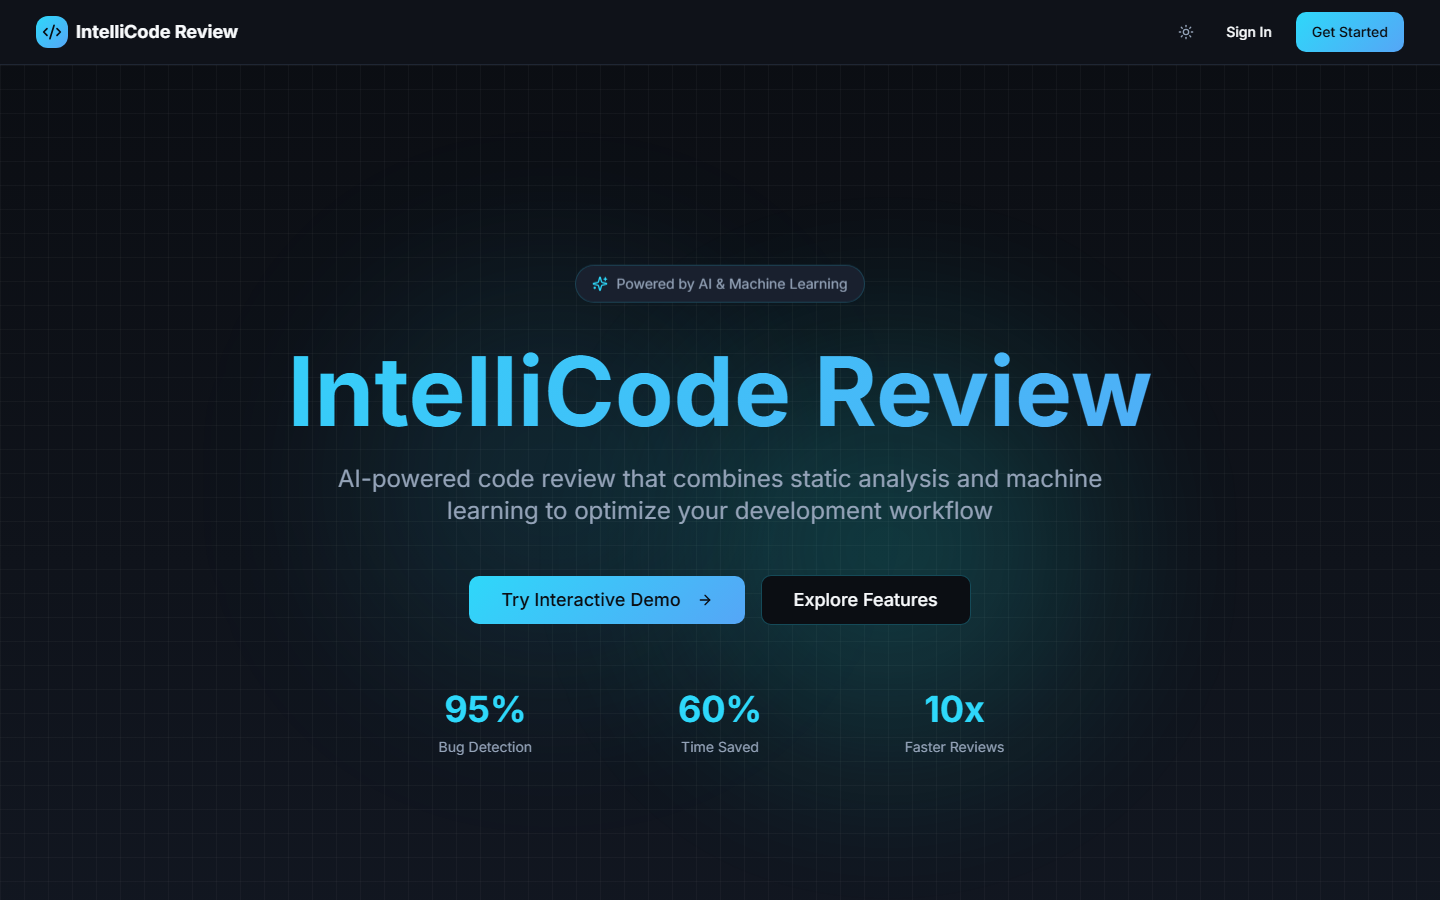
\includegraphics[width=0.95\linewidth]{01_landing.png}
\caption{Landing page of the running IntelliCode Review prototype. The hero section displays three aspirational headline figures used in the interface copy, and provides direct access to the embedded demo and feature overview. These figures reflect the platform's intended positioning and are not derived from controlled user experiments.}
\label{fig:landing}
\end{figure}

%% ============================================================

\chapter{Software Design and Implementation}
\label{ch:design}


\chapter{Prototype Demonstration}
\label{ch:demo}


\chapter{Validation and Evaluation}
\label{ch:eval}


\chapter{Conclusion}
\label{ch:conclusion}

\end{document}
